\documentclass[10pt,twocolumn]{article}
\usepackage[letterpaper,margin=0.72in,columnsep=0.25in]{geometry}
\usepackage[T1]{fontenc}
\usepackage{lmodern}
\usepackage{amsmath,amssymb,amsthm,booktabs,array,tabularx}
\usepackage{graphicx,xcolor,microtype,tikz,pgfplots,enumitem,hyperref}
\pgfplotsset{compat=1.18}
\usetikzlibrary{arrows.meta,positioning}
\hypersetup{colorlinks=true,linkcolor=blue!55!black,citecolor=blue!55!black,urlcolor=blue!55!black,
 pdftitle={S1Q: Low-Bit Quantization for System One Decision Models},pdfauthor={Yuanming Chen}}
\setlength{\textfloatsep}{10pt plus 2pt minus 2pt}
\setlength{\floatsep}{9pt plus 2pt minus 2pt}
\setlength{\abovecaptionskip}{5pt}
\setlist{nosep,leftmargin=*}
\newcommand{\E}{\mathbb E}
\newcommand{\R}{\mathbb R}
\newcommand{\diag}{\operatorname{diag}}
\newcommand{\clip}{\operatorname{clip}}
\newcommand{\softmax}{\operatorname{softmax}}
\newcommand{\JS}{\operatorname{JS}}
\newcommand{\KL}{\operatorname{KL}}
\newcommand{\sg}{\operatorname{stopgrad}}
\newtheorem{proposition}{Proposition}
\newcommand{\repo}{\href{https://github.com/CYMCharming/S1Q}{github.com/CYMCharming/S1Q}}
\title{\vspace{-0.6cm}\textbf{S1Q: Low-Bit Quantization for\\System One Decision Models}}
\author{Yuanming Chen\\\small \href{https://github.com/CYMCharming}{CYMCharming}}
\date{\small October 1, 2026\\\footnotesize Research manuscript draft; experimental snapshot v0.1.0}
\begin{document}
\maketitle
\begin{abstract}
Typed decision models map a state and structured questions directly to
distributions over supplied choices, Boolean answers, or ordered score levels.
Their deployment calls for quantization evaluations that measure decision
and probability preservation in addition to storage.
We present S1Q, an open post-training quantization framework that adapts
activation-aware channel scaling and groupwise clipping to native decision
interfaces, with an optional label-free categorical-Fisher sensitivity
estimator. A held-out development objective selects among weight-only,
selectively protected, and simulated activation-quantized profiles.
We evaluate Kev-0.8B, Kev-4B, Kev-9B, NanoJev, and Laya, spanning hybrid
decoder, decoder-only, and encoder architectures. On exploratory main cohorts,
selected S1Q improves or ties matched round-to-nearest quantization; four of
five paired 95\% intervals include zero. A separate fixed-profile evaluation
on 85 screened public JevBench tasks yields heterogeneous outcomes, with all
five improvement intervals including zero. Estimated complete parameter
storage falls by 48.4--70.6\%, and measured persistent CUDA allocations fall
by 48.2--69.4\%. Packed execution still performs floating-point matrix
multiplication, so these reductions do not establish integer-kernel
acceleration. S1Q contributes native adapters, explicit sensitivity and
selection procedures, pinned evaluation recipes, and a reproducible account
of both gains and failures.
\end{abstract}

\section{Introduction}
Many model-mediated decisions have a finite output space: authorize or deny
a request, choose one supplied action, or assign a discrete score.
The System One model paradigm and Jev's typed API motivate direct prediction
of such distributions rather than an autoregressive answer trace
\cite{typesafe2026jev}. Independent open implementations include Kev,
NanoJev, and Laya \cite{palmer2026kev,tianyu2026nanojev,kishor2026laya}.
We use \emph{System One decision model} operationally for this interface,
not as a claim that these models share a standardized architecture.
The hosted TypeSafe Jev service is not an open checkpoint evaluated here.

Low-bit quantization is a practical way to reduce parameter storage.
Strong language-model methods include GPTQ, AWQ, SmoothQuant, and
OmniQuant \cite{frantar2023gptq,lin2024awq,xiao2023smoothquant,shao2024omniquant}.
However, a deployment decision can change when the two leading candidate
probabilities are close, even if an aggregate reconstruction error is small.
Conversely, preserving an original model's probabilities does not imply
that those probabilities describe empirical truth well. A decision-focused
study must distinguish accuracy, fidelity to the native model, label-based
probability quality, and system resource use.

Architecture and interface details also matter. Kev combines a Qwen
hybrid backbone, merged adapters, and a pointer head. NanoJev uses a
Qwen3 backbone with dynamic candidate heads. Laya uses a ModernBERT
encoder and typed heads. Candidate numbers vary by question, and a
request can contain multiple questions. Generic causal-language-model
evaluation or a rewritten prompt can silently change the task.
We quantize through pinned native adapters and retain each
implementation's admitted question encoding and candidate order.

S1Q adapts established groupwise quantization, activation-aware scaling,
and clipping search to these interfaces. Its optional Fisher variant
estimates how intermediate perturbations affect the teacher's categorical
decision distribution. Random projections accommodate variable candidate
sets without constructing a full propagated Fisher matrix. A finite
development search chooses the entire profile rather than assuming
that additional sensitivity weighting or lower activation precision always
helps. We do not claim that scaling, clipping, Fisher sensitivity, or
protected heads are individually new.

The empirical findings are mixed. Main-cohort accuracy differences against
matched RTN are nonnegative, but most confidence intervals include zero.
Source transfer includes losses, and an external authored cohort does not
show consistent improvement. Raw main negative log-likelihood is worse
than RTN for four of five models. The Fisher variant is selected for only
one model. These observations motivate a conservative account of what
decision-aware quantization preserves and what it can damage.

Our contributions are:
\begin{enumerate}
 \item A native PTQ framework and cross-architecture study of five
 released decision checkpoints, with explicit quantized and retained
 module boundaries.
 \item A specified adaptation combining input second moments, optional
 categorical-Fisher probes, groupwise scale/clipping search, and
 development-based decision preservation.
 \item Paired accuracy, probability, transfer, and storage analyses,
 including an externally frozen authored cohort and disclosed negative results.
 \item Pinned recipes, paired predictions, and packed linear artifacts
 where redistribution is permitted, with measured persistent-memory
 reductions separated from unimplemented integer-kernel acceleration.
\end{enumerate}
Code and artifacts are available at \repo.

\section{Related Work}
\paragraph{Post-training quantization.}
GPTQ uses approximate second-order reconstruction and error compensation
\cite{frantar2023gptq}. AWQ motivates activation-guided channel scaling
\cite{lin2024awq}, while SmoothQuant uses equivalent transformations to
support weight--activation quantization \cite{xiao2023smoothquant}.
OmniQuant learns clipping and equivalent transformations through
reconstruction \cite{shao2024omniquant}. S1Q uses a small discrete
grid and a factorized diagonal proxy; it is neither an official
reproduction of these algorithms nor evidence of superiority to them.
Rotation-based approaches, including QuaRot and SpinQuant, and
W4A8 systems such as QQQ illustrate the separate roles of
numerical conditioning and efficient kernels
\cite{ashkboos2024quarot,liu2024spinquant,zhang2024qqq}.

\paragraph{Sensitivity and uncertainty.}
Fisher-based quantization sensitivity has been studied by FIT
\cite{zandonati2023fit}. GuidedQuant incorporates end-loss guidance
\cite{kim2025guidedquant}. C-PTQ uses Fisher-weighted channel sensitivity
and is especially close to the motivation for S1Q's optional row weights
\cite{li2026cptq}. We treat Fisher weighting as established prior art;
our implementation adapts teacher categorical probes and question
normalization to native typed decisions.
DPQ targets uncertainty through calibration-data selection
\cite{yang2026dpq}. S1Q's development objective uses decision margins
and probability drift, but does not implement DPQ's data-selection
procedure. Temperature scaling is a separate probability-calibration
operation \cite{guo2017calibration}.

\paragraph{Quantized decision models.}
Public Laya INT4 ONNX artifacts, Laya MLX engineering experiments,
Kev INT8 evaluations, and quantized Kev GGUF backbones precede this study
\cite{androidli2026laya,mizore2026laya,kev2026issue162,dreamblooms2026kev}.
Thus S1Q is not the first quantization of this model class.
Different revisions, tasks, temperatures, and runtimes prevent treating
their reported values as controlled S1Q comparisons. Our emphasis is a
common audited procedure with native interfaces, paired probability
measurements, and explicit failure disclosure.

\section{Problem and Evaluation Contract}
A request contains a state and $Q$ typed questions. Question $q$ has a
finite candidate set of size $K_q$ and teacher logits
$z_q\in\R^{K_q}$. A Boolean question uses the common ordering
$[\mathrm{false},\mathrm{true}]$; NanoJev's native scalar Boolean logit
$z$ is represented as $[0,z]$. Choice insertion order is retained.
Score levels are treated as categories for the Fisher calculation;
ordinal expected-level error is reported separately.

Let $\theta$ denote the original checkpoint and $\widehat\theta$ the
quantized model. We seek low parameter storage while preserving native
decision behavior. This is not a guarantee that the teacher is correct
or calibrated. Task labels are used for final scoring and development
selection, but are removed from inference inputs and from PTQ statistic
collection.

We quantize supported backbone $\mathrm{Linear}$ weights.
Embeddings, decision heads, normalization, biases, convolution,
and recurrent-state arithmetic retain their loaded precision.
Shared parameters crossing the boundary are rejected rather than
silently changing a protected module. Kev adapters are merged before
collecting statistics. Each compared method uses the same admitted
records and candidate semantics; inputs are not truncated to rescue
a failed quantized prediction.

\section{S1Q Method}
\begin{figure*}[t]
\centering
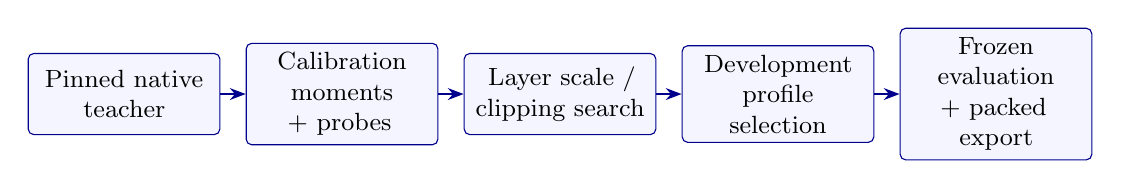
\begin{tikzpicture}[
 box/.style={draw=blue!55!black,fill=blue!4,rounded corners=2pt,
 text width=2.2cm,minimum height=1.03cm,align=center,font=\small},
 arr/.style={-{Stealth[length=2mm]},thick,blue!55!black}]
\node[box] (a) {Pinned native\\teacher};
\node[box,right=0.32cm of a] (b) {Calibration\\moments + probes};
\node[box,right=0.32cm of b] (c) {Layer scale /\\clipping search};
\node[box,right=0.32cm of c] (d) {Development\\profile selection};
\node[box,right=0.32cm of d] (e) {Frozen evaluation\\+ packed export};
\draw[arr] (a)--(b); \draw[arr] (b)--(c); \draw[arr] (c)--(d); \draw[arr] (d)--(e);
\end{tikzpicture}
\caption{S1Q separates calibration statistics, local quantizer search,
whole-model development selection, and fixed-profile evaluation.
PTQ moments and probes are label-free; development selection and
optional probability-temperature fitting use separate labeled partitions.}
\label{fig:pipeline}
\end{figure*}

\subsection{Input Second Moments}
For a layer $y=Wx+b$, $W\in\R^{d_{\mathrm{out}}\times d_{\mathrm{in}}}$,
collect the pristine teacher's input activations on calibration requests.
Flatten leading dimensions into rows and compute
\begin{equation}
 m_j=\E_{\mathrm{cal}}[x_j^2],\quad
 h_j=\frac{m_j}{\max(\operatorname{mean}_k m_k,10^{-30})}.
 \label{eq:input}
\end{equation}
These are \emph{uncentered} second moments, not a centered covariance.
The collector includes padding rows emitted by the native forward.
Normalization does not change candidate ordering within a layer.

\subsection{Optional Categorical-Fisher Probes}
At fixed $T>0$, define
\begin{equation}
 u_q=z_q/T,\quad p_q=\softmax(u_q),\quad
 F_q=\diag(p_q)-p_qp_q^\top .
 \label{eq:fisher}
\end{equation}
$F_q$ is the categorical Fisher in scaled-logit coordinates.
It uses the teacher distribution, not a gold label or a task reward.
For independent $\epsilon_q\sim\mathcal N(0,I_{K_q})$, set
\begin{align}
 a_q&=\diag(\sqrt{p_q})\epsilon_q,\\
 v_q&=a_q-p_q\mathbf 1^\top a_q,\\
 \ell_{\mathrm{probe}}&=Q^{-1/2}\sum_q \sg(v_q)^\top u_q .
 \label{eq:probe}
\end{align}
$p_q$ and $v_q$ are detached during differentiation.
The scalar is a device for collecting sensitivity, not a training loss
that is minimized.

\begin{proposition}[Conditional probe covariance]
Fix a teacher, a calibration record, and a differentiable intermediate
output $y$, vectorized across token rows and channels.
Write $J_q=\partial u_q/\partial y$ and
$g=\nabla_y\ell_{\mathrm{probe}}$. Then
\begin{align}
 \E[v_q]&=0,\quad \E[v_qv_q^\top]=F_q,\\
 \mathbf 1^\top v_q&=0,\quad \E[g]=0,\\
 \E[gg^\top]&=Q^{-1}\sum_q J_q^\top F_qJ_q .
 \label{eq:propagated}
\end{align}
\label{prop:cov}
\end{proposition}
The $Q^{-1/2}$ factor makes the expected squared gradient correspond
to question-averaged sensitivity within a request. The common-shift
identity removes sensitivity to adding the same constant to every
candidate logit. It does not imply independence of token rows or
independence of the questions' representations.

For output channel $i$, accumulate squared gradients over records,
probes, and flattened output rows:
\begin{equation}
 \widehat f_i=
 \frac{\sum_r\sum_{k=1}^P\sum_{t=1}^{n_r}
       (g_{r,k})_{ti}^{\,2}}
      {P\sum_r n_r}.
 \label{eq:moment}
\end{equation}
For a nonzero estimate, the implemented row weight is
\begin{equation}
 r_i=\max\left(
 \frac{\widehat f_i}{\max(\operatorname{mean}_k\widehat f_k,10^{-30})},
 10^{-4}\right).
 \label{eq:row}
\end{equation}
An all-zero estimate and the activation-only variant use $r_i=1$.
There is no renormalization after the floor.
The normalized, floored weight is not an unbiased Fisher estimate;
the covariance property applies to the raw probes and squared gradients.
Parameters are frozen during collection, so backward passes do not
update them. Failed records discard all partial statistics and do
not trigger a silent activation-only fallback.

\subsection{Equivalent Scaling and Groupwise Quantization}
For exponent $\alpha$, preliminary observed-channel scales are
$\widetilde s_j=\max(\sqrt{h_j},10^{-8})^\alpha$.
Normalize by the geometric midpoint of the observed minimum and maximum,
then clamp to $[10^{-4},10^4]$. Unobserved channels receive one;
$\alpha=0$ sets every scale to one. With $S_\alpha=\diag(s)$,
\begin{equation}
 W'_\alpha=WS_\alpha,\qquad x'_\alpha=S_\alpha^{-1}x .
\end{equation}
This preserves $Wx+b$ before rounding in exact arithmetic.

Groups run along the input dimension independently in each output row,
with default group size 128 and zero padding of a final incomplete group.
For bit width $b$, clipping ratio $c$, and group $g$:
\begin{align}
 q_{\max}&=2^{b-1}-1,\\
 d_{ig}&=\frac{c\max_{j\in g}|(W'_\alpha)_{ij}|}{q_{\max}},\\
 q_{ij}&=\clip\!\left(
  \operatorname{round}\frac{(W'_\alpha)_{ij}}{d_{ig}},
  -q_{\max},q_{\max}\right).
 \label{eq:quant}
\end{align}
All-zero groups use $d_{ig}=1$. No affine zero point is stored.
W4 uses $[-7,7]$ and W8 uses $[-127,127]$; the unused most-negative
code is intentional. Clipping rescales a group's maximum absolute
range; it is not a percentile filter or removal of a fraction of weights.
Define the reconstructed effective weight
\begin{equation}
 \widehat W_{\alpha,c}
 =\mathcal Q_{b,c}(WS_\alpha)S_\alpha^{-1}.
\end{equation}

\subsection{Local Reconstruction Objective}
Each layer independently minimizes
\begin{equation}
 E_\ell(\alpha,c)=
 \sum_{i,j}r_i h_j
 \big((\widehat W_{\alpha,c})_{ij}-W_{ij}\big)^2
 \label{eq:local}
\end{equation}
over $\alpha\in\{0,0.25,0.5,0.75\}$ and
$c\in\{0.9,0.95,1\}$. Exact ties prefer smaller $\alpha$, then larger $c$.
The 12-point grid includes RTN at $(\alpha,c)=(0,1)$.
RTN performs no calibration-based search.
The activation-only profile sets $r_i=1$.

Equation~\eqref{eq:local} has a local motivation. For a small scaled-logit
perturbation $\delta u_q$,
\begin{equation}
 \KL(p_q\|\softmax(u_q+\delta u_q))
 =\tfrac12\delta u_q^\top F_q\delta u_q
 +O(\|\delta u_q\|^3).
\end{equation}
Local linearization gives $\delta u_q\approx J_q\delta y$.
For a single layer with teacher inputs held fixed,
$\delta y=\Delta W x$. Dropping output-channel, token-position, and
input-channel cross terms, and factorizing activation magnitude from
output sensitivity, motivates a term proportional to
$\sum_{ij}\E[H_{ii}]\E[x_j^2](\Delta W_{ij})^2$, where
$H=Q^{-1}\sum_qJ_q^\top F_qJ_q$.
The moment normalizations and sensitivity floor further modify this proxy.
Cross-layer interactions and changes to downstream inputs are omitted.
Thus the exact covariance in Proposition~\ref{prop:cov} does not make
the diagonal reconstruction objective exact or guarantee task gains.

\subsection{Protection and Activation Profiles}
Optional protection ranks eligible layers by calibrated RTN relative error:
\begin{equation}
 \rho_\ell=
 \frac{\sum_{ij}r_i h_j
    (\widehat W^{\mathrm{RTN}}_{ij}-W_{ij})^2}
      {\sum_{ij}r_i h_jW_{ij}^2}.
\end{equation}
A zero denominator yields zero. Preserve the largest
$\lceil\eta L\rceil$ scores, breaking ties by module name;
the tested $\eta$ is 0.05. This budget counts layers, not parameters.
The native protected boundary remains in effect even when $\eta=0$.

Optional A4/A8 applies dynamic symmetric quantize--dequantize (QDQ) to
each selected linear input row \emph{after} compensation.
One scale per row is its maximum absolute feature value divided by
7 or 127. Values are rounded, clamped, and immediately reconstructed
in the original floating dtype. Other activations and recurrent states
remain native. This is numerical simulation, not an integer activation
runtime or KV-cache quantization.

\subsection{Whole-Model Development Selection}
Each profile starts from the pristine teacher and uses either uniform
or Fisher output weights. Profiles are RTN, local, local with protection,
local with A8/A4 QDQ, and, when enabled, Fisher with or without protection.
There is no Fisher-plus-A4/A8 candidate in the current grid.
RTN is a baseline, not a candidate for the selected S1Q label.

For development question $n$, let $p_n$ and $\widehat p_n$ be probabilities
from raw teacher and quantized logits at temperature one. Let $m_n$ be
the difference of the teacher's largest two probabilities:
\begin{align}
 w_n&=1+\clip((0.2-m_n)/0.2,0,1),\\
 \mathcal J_{\mathrm{dev}}
 &=\frac{\sum_n w_n\JS(p_n,\widehat p_n)}{\sum_n w_n}
   +\frac{0.1}{N}\sum_n H_n ,
 \label{eq:dev}\\
 H_n&=\mathbf 1[
   \arg\max p_n=y_n,\ 
   \arg\max\widehat p_n\ne y_n].
\end{align}
The weight lies in $[1,2]$ and emphasizes near-boundary decisions.
The harmful-flip term uses development labels; S1Q is not entirely
label-free. Only exact objective ties are broken by estimated complete
packed parameter bytes. The selection is persisted before evaluating
quantized test cohorts. Reporting temperatures are fitted separately
and do not enter Equation~\eqref{eq:dev}.

\begin{figure}[t]
\small
\fbox{\begin{minipage}{0.94\columnwidth}
\textbf{Algorithm 1: S1Q}
\begin{enumerate}
 \item Pin the teacher and native adapter; freeze candidate ordering,
 module boundary, admitted records, and data partitions.
 \item Collect input moments; optionally collect categorical-Fisher
 output moments from the unchanged teacher.
 \item For each profile, rank optional protected layers, then search
 $(\alpha,c)$ independently in remaining linears.
 \item Evaluate compensated reconstructed weights and optional
 activation QDQ on development requests.
 \item Select the S1Q profile minimizing $\mathcal J_{\mathrm{dev}}$;
 persist its layer policy and parameters.
 \item Fit separate reporting temperatures; evaluate frozen profiles
 on paired test, transfer, and external cohorts.
 \item Pack integer codes and save scales, module identities,
 model pins, and hashes.
\end{enumerate}
\end{minipage}}
\caption{Calibration controls local quantizer parameters; development
controls the whole-model profile. External data controls neither.}
\label{fig:algorithm}
\end{figure}

\subsection{Storage and Reference Execution}
W4 packs two signed nibbles into each byte. Artifacts contain integer
payloads, FP32 group scales, and input-channel scales. Biases,
retained native weights, architecture, heads, and tokenizer are obtained
from the pinned native checkpoint. An artifact is a packed
linear derivative, not a standalone compressed checkpoint.

The reversible accuracy path reconstructs floating weights and does
not reduce their tensor dtype. The packed runtime instead replaces
selected modules with integer buffers and transiently dequantizes
one matrix per call before floating $\mathrm{Linear}$ computation.
It has no INT4/INT8 GEMM kernel. Loading first constructs the full
native model; measured inference peaks exclude that initial allocation.
Functional callers that directly access a reconstructed weight can bypass
the A4/A8 input hook, so architecture coverage requires native parity checks.

\section{Experimental Setup}
\paragraph{Models and hardware.}
We evaluate three Kev sizes, NanoJev, and Laya at immutable source
and checkpoint revisions (Appendix~\ref{app:pins}).
Kev experiments use an A100 80GB GPU; NanoJev and Laya use an
A800 80GB GPU. Kev backbones are stored in BF16 with native
FP32 head components. NanoJev and Laya native parameters are
FP32 with BF16 autocast computation; a BF16 compute flag does
not imply that their baseline parameter storage is BF16.
Recorded package versions and a separately tested supported CPU profile
are distinguished in Appendix~\ref{app:runtime}.

\paragraph{Quantizer budget.}
The main study fixes W4, group size 128, and the native head policy.
It does not optimize bit width globally. All five completed expanded
runs consider the optional Fisher profiles, using two probes per
request and up to 32 accepted calibration requests at $T=1$.
Input statistics use the frozen calibration set. Local candidate
reconstruction uses FP32, followed by execution in native compute
dtypes. The protected profiles retain 5\% of eligible layers.
W8 support is available in code but is not an executed supplementary
comparison in this snapshot.

\paragraph{Data.}
The shared screened Kev decision-v7 test has 711 requests, 914
questions, and 631 clusters; source-transfer-v4 has 630 requests/questions
and 518 clusters. The shared quantizer, temperature, and development
partitions have respectively 128/155, 128/155, and 256/311
requests/questions. Decision-v7 mixes public text tasks and deterministic
rule scenarios and shares source families with Kev's supervision.
Transfer source families are held out from Kev supervision, not certified
unseen by every other model.

NanoJev's evaluated native-release cohorts contain \emph{only shooting}
states. Test has 1,023 decisions in 102 episode components, and OOD
has 1,024 in 150 components. Every evaluated label is marked
\texttt{reference\_argmax\_compatibility}: it is a supplied argmax
action from an upstream visual reference policy. These are neither
human judgments nor observed success probabilities. The converter
copies explicitly supplied gold; it does not manufacture gold from
S1Q or teacher predictions. The broader upstream package also contains
other games, but those are not the final evaluated cohorts.

The independent external source is specifically
\texttt{fstandhartinger/jevbench} \cite{standhartinger2026jevbench}.
A declared maximum of 10 candidates and 1,000 complete-request
characters admits 85 of 183 public original-plus-hard tasks:
72 original and 13 hard, in 49 scenario clusters. Ninety-eight hard
tasks are excluded for length. The retained questions comprise
40 Choice, 33 Boolean, and 12 Score tasks. Hard labels have
model-assisted authorship and cross-review. No additional native
adapter exclusions occur for these five external runs.
This is a screened public authored cohort, not the full benchmark
or a leaderboard result.

\paragraph{Split and development disclosure.}
Exact public requests and source groups are checked across partitions.
NanoJev episodes linked by duplicate requests are joined into components;
lower-priority overlapping components are removed whole before sampling.
This does not establish absence of paraphrase duplicates or unknown
pretraining contamination.
Early Laya pilot test/transfer results informed the Fisher extension.
Expanded main, transfer, and game OOD evaluations reuse overlapping
inspected sources and remain exploratory. The external study freezes
selection, artifacts, calibration policy, and data hashes before its
first prediction and performs no external fitting or tuning.

\paragraph{Comparisons and metrics.}
We compare native checkpoints, matched RTN, an unprotected local
ablation, and selected S1Q. RTN matches weight format, group size,
quantized tensor identities, protection, and activation scheme.
Kev-9B uses A8-matched RTN rather than ordinary W4 RTN.
Official AWQ/GPTQ/OmniQuant experiments are absent; the local ablation
must not be relabeled an official implementation.
We report accuracy, NLL, multiclass Brier, 15-bin top-label ECE,
JS drift, harmful flips, and score expected-level MAE.
Paired percentile cluster bootstrap uses 2,000 resamples and
seed 20261001. It is not source-stratified and has no
multiple-comparison correction.

\section{Results}
\begin{table*}[t]
\centering\footnotesize
\setlength{\tabcolsep}{3.5pt}
\begin{tabular}{llrrrrll}
\toprule
Model & Selected policy & $n$ & Native & RTN & S1Q
 & $\Delta$ vs.\ RTN [95\% CI] & $\Delta$ vs.\ native [95\% CI]\\
\midrule
Kev-0.8B & Fisher W4 & 914 & 82.93 & 80.63 & 81.18 & $+0.55 [-1.07, +2.18]$ & $-1.75 [-3.06, -0.45]$ \\
Kev-4B & Local W4 & 914 & 85.45 & 84.79 & 84.79 & $+0.00 [-1.36, +1.30]$ & $-0.66 [-1.76, +0.43]$ \\
Kev-9B & Local W4A8$^{\dagger}$ & 914 & 86.98 & 84.35 & 86.54 & $+2.19 [+0.76, +3.71]$ & $-0.44 [-1.44, +0.55]$ \\
NanoJev & Local W4 & 1023 & 79.86 & 79.47 & 80.45 & $+0.98 [-0.11, +2.31]$ & $+0.59 [-0.30, +1.48]$ \\
Laya & Local W4 & 914 & 66.85 & 63.68 & 64.55 & $+0.88 [-1.27, +3.10]$ & $-2.30 [-4.25, -0.23]$ \\
\bottomrule
\end{tabular}
\caption{Exploratory main-cohort accuracy (\%). Differences and interval
endpoints are percentage points. Kev/Laya use the shared 914-question
cohort; NanoJev uses 1,023 reference-policy action targets.
$^\dagger$A8 is simulated QDQ and is matched in RTN.
Intervals describe paired differences, not absolute-accuracy uncertainty.}
\label{tab:main}
\end{table*}

\subsection{Main Accuracy and Native Loss}
Selected S1Q improves or ties matched RTN on the main cohorts
(Table~\ref{tab:main}), but four of five difference intervals include zero.
Kev-9B gains 2.19 percentage points, with an interval of
$[0.76,3.71]$. These inspected, expanded experiments are exploratory;
this interval is not an independent confirmation of a general gain.
Kev-0.8B and Laya lose 1.75 and 2.30 points against native checkpoints,
respectively. Their descriptive native-difference intervals are entirely
negative. W4 is therefore not lossless, and the data do not support
uniform noninferiority to native inference.

\begin{figure*}[t]
\centering
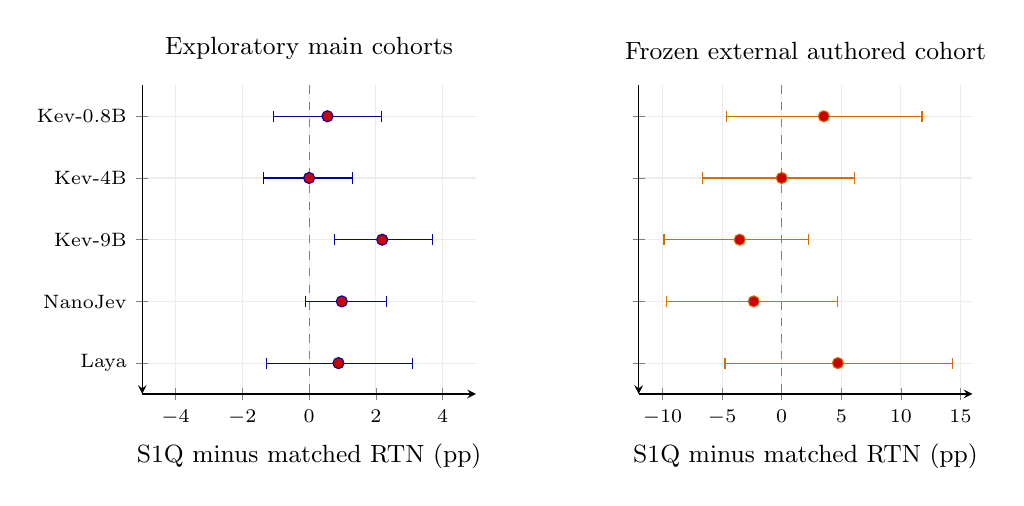
\begin{tikzpicture}
\begin{axis}[
 width=0.48\textwidth,height=5.5cm,title={Exploratory main cohorts},
 xmin=-5,xmax=5,xtick={-4,-2,0,2,4},
 ymin=0.5,ymax=5.5,y dir=reverse,ytick={1,2,3,4,5},
 yticklabels={Kev-0.8B,Kev-4B,Kev-9B,NanoJev,Laya},
 xlabel={S1Q minus matched RTN (pp)},
 tick label style={font=\scriptsize},label style={font=\small},
 title style={font=\small},grid=major,grid style={gray!15},axis lines=left]
\addplot[gray,dashed] coordinates {(0,0.5)(0,5.5)};
\addplot+[only marks,mark=*,blue!65!black,error bars/.cd,x dir=both,x explicit]
 table[row sep=\\,x=x,y=y,x error plus=plus,x error minus=minus] {
x y plus minus\\
0.55 1 1.63 1.62\\
0.00 2 1.30 1.36\\
2.19 3 1.52 1.43\\
0.98 4 1.33 1.09\\
0.88 5 2.22 2.15\\
};
\end{axis}
\begin{axis}[
 at={(0.52\textwidth,0)},anchor=south west,width=0.48\textwidth,height=5.5cm,
 title={Frozen external authored cohort},
 xmin=-12,xmax=16,xtick={-10,-5,0,5,10,15},
 ymin=0.5,ymax=5.5,y dir=reverse,ytick={1,2,3,4,5},yticklabels={,,,,},
 xlabel={S1Q minus matched RTN (pp)},
 tick label style={font=\scriptsize},label style={font=\small},
 title style={font=\small},grid=major,grid style={gray!15},axis lines=left]
\addplot[gray,dashed] coordinates {(0,0.5)(0,5.5)};
\addplot+[only marks,mark=*,orange!85!black,error bars/.cd,x dir=both,x explicit]
 table[row sep=\\,x=x,y=y,x error plus=plus,x error minus=minus] {
x y plus minus\\
3.53 1 8.24 8.13\\
0.00 2 6.10 6.67\\
-3.53 3 5.75 6.35\\
-2.35 4 7.06 7.29\\
4.71 5 9.58 9.47\\
};
\end{axis}
\end{tikzpicture}
\caption{Paired 95\% cluster-bootstrap intervals. The external panel uses
a wider horizontal scale because the small cohort has greater uncertainty.
Every external interval crosses zero; neither consistent improvement
nor equivalence follows. Cohort definitions and profiles remain distinct.}
\label{fig:intervals}
\end{figure*}

\subsection{Transfer and Native-Release OOD}
Transfer results are heterogeneous (Table~\ref{tab:transfer}).
Kev-4B gains 2.06 points over matched RTN, while Kev-0.8B
loses 2.38 and Kev-9B loses 0.16. NanoJev's game OOD gain is
0.88 points with an interval spanning zero. A smaller local surrogate
or better main-cohort fidelity does not guarantee better
accuracy under source or domain shift.

\begin{table*}[t]
\centering\small
\begin{tabular}{lrrrrl}
\toprule
Model & $n$ & Native & RTN & S1Q & $\Delta$ vs.\ RTN [95\% CI]\\
\midrule
Kev-0.8B & 630 & 68.25 & 68.25 & 65.87 & $-2.38 [-5.38, +0.48]$ \\
Kev-4B & 630 & 83.97 & 83.17 & 85.24 & $+2.06 [+0.16, +4.10]$ \\
Kev-9B & 630 & 85.24 & 84.44 & 84.29 & $-0.16 [-1.79, +1.57]$ \\
Laya & 630 & 66.03 & 65.87 & 66.83 & $+0.95 [-1.93, +3.93]$ \\
\midrule
NanoJev & 1024 & 77.44 & 76.95 & 77.83 & $+0.88 [-0.09, +1.86]$ \\
\bottomrule
\end{tabular}
\caption{Exploratory source transfer (Kev/Laya) and native-release game
OOD (NanoJev). Accuracy is \%; differences are pp.
Transfer uses 518 clusters; NanoJev OOD uses 150 episode components.
Source holdout is defined relative to Kev supervision.}
\label{tab:transfer}
\end{table*}

\subsection{Frozen External Evaluation}
On the screened JevBench cohort, selected-minus-RTN differences
range from $-3.53$ to $+4.71$ points
(Table~\ref{tab:external}, Figure~\ref{fig:intervals}).
All five paired intervals include zero. Point estimates include
gains, a tie, and losses; this small authored set does not establish
consistent cross-model improvement. An interval crossing zero is
also not evidence of equivalence.

NanoJev's native general-domain accuracy is already 40.00\%;
S1Q yields 38.82\%, a further $-1.18$-point change.
The low absolute native score is consistent with a transfer limitation before
quantization, while the paired difference isolates an additional
quantizer effect. We do not infer general-purpose decision ability
from its specialized shooting-game evaluation.

\begin{table*}[t]
\centering\small
\begin{tabular}{lrrrrl}
\toprule
Model & $n$ & Native & RTN & S1Q & $\Delta$ vs.\ RTN [95\% CI]\\
\midrule
Kev-0.8B & 85 & 76.47 & 72.94 & 76.47 & $+3.53 [-4.60, +11.77]$ \\
Kev-4B & 85 & 88.24 & 84.71 & 84.71 & $+0.00 [-6.67, +6.10]$ \\
Kev-9B & 85 & 83.53 & 88.24 & 84.71 & $-3.53 [-9.88, +2.22]$ \\
NanoJev & 85 & 40.00 & 41.18 & 38.82 & $-2.35 [-9.64, +4.71]$ \\
Laya & 85 & 64.71 & 61.18 & 65.88 & $+4.71 [-4.76, +14.29]$ \\
\bottomrule
\end{tabular}
\caption{Fixed-profile external JevBench authored cohort: 85 tasks in
49 clusters, with 98 long hard tasks excluded by the declared screen.
No profile, temperature, or quantizer fitting uses this cohort.
Accuracy is \%; differences are pp.}
\label{tab:external}
\end{table*}

\subsection{Ablations and Probability Quality}
Fisher is selected for only Kev-0.8B; the other four models choose
local activation-aware scaling, with Kev-9B adding A8 QDQ.
No selected profile retains the optional extra 5\% of layers.
The development grid does not establish a general Fisher
benefit. Full development accuracy and objective values are reported
in Appendix~\ref{app:ablation}.

A4 QDQ reduces development accuracy relative to native for every model.
The drops are large for the Kev checkpoints and Laya, but much smaller
for NanoJev. This motivates model-specific activation checks,
not a successful universal W4A4 recipe.

Raw main NLL is worse than matched RTN for Kev-0.8B, Kev-4B,
Kev-9B, and Laya. Accuracy or teacher fidelity can improve while
label-based probability quality degrades.
Temperature fitting is offered to every compared method on its
separate labeled partition; it does not change argmax accuracy.
Appendix~\ref{app:probability} reports raw and temperature-scaled NLL,
Brier, and ECE. None establishes real-world event
calibration for authored or reference-policy targets.

\subsection{Storage and Persistent Memory}
Estimated complete parameter storage, including retained native
components and quantizer auxiliaries, is 29.4--51.6\% of native
storage (Table~\ref{tab:storage}). The denominator reflects actual
native storage precision, not a uniform hypothetical FP16 model.
Quantized parameter coverage varies from 66.09\% to 87.15\%.
A small exported linear file should not be reported as the
complete-model compression ratio.

\begin{table}[t]
\centering\footnotesize
\setlength{\tabcolsep}{3pt}
\begin{tabular}{lrrrr}
\toprule
Model & Q.\ \% & Native & Packed & Ratio \%\\
\midrule
Kev-0.8B & 66.09 & 1437.1 & 741.1 & 51.6 \\
Kev-4B & 84.84 & 8026.8 & 3031.0 & 37.8 \\
Kev-9B & 87.15 & 15146.0 & 5460.1 & 36.0 \\
NanoJev & 73.86 & 2274.5 & 818.7 & 36.0 \\
Laya & 81.45 & 1607.1 & 472.6 & 29.4 \\
\bottomrule
\end{tabular}
\caption{Parameter storage estimates in MiB. Packed includes
retained native parameters and scales; Q.\ \% is quantized parameter
coverage. This is not a device-memory measurement.}
\label{tab:storage}
\end{table}

Measured persistent PyTorch CUDA allocation decreases by 48.2--69.4\%
(Table~\ref{tab:runtime}). For Kev-9B it falls from 15,154.2 to
5,488.1 MiB, with a packed inference peak of 6,107.1 MiB.
The initial full native checkpoint load is excluded from that peak,
so these figures do not establish direct loading on a device of
the packed persistent size.

\begin{table}[t]
\centering\footnotesize
\setlength{\tabcolsep}{3pt}
\begin{tabular}{lrrrr}
\toprule
Model & $n$ & Dense & Packed & Peak\\
\midrule
Kev-0.8B & 41 & 1469.2 & 760.5 & 881.0 \\
Kev-4B & 41 & 8131.0 & 3123.0 & 3503.8 \\
Kev-9B & 41 & 15154.2 & 5488.1 & 6107.1 \\
NanoJev & 32 & 2284.4 & 832.2 & 946.8 \\
Laya & 41 & 1616.5 & 495.1 & 551.8 \\
\bottomrule
\end{tabular}
\caption{Measured allocated CUDA memory (MiB) after conversion:
dense/packed persistent allocation and packed inference peak.
$n$ counts scored parity decisions. Each packed path has zero measured
JS and decision flips against the same artifact's dense reconstruction
on this small subset.}
\label{tab:runtime}
\end{table}

Parity checks cover 41 scored decisions for each Kev model and Laya,
and 32 for NanoJev. Zero JS and flips on these subsets do not establish
bitwise equality or full-test packed validation.
The benchmark records packed request times but lacks paired dense
latency measurements; we report no speedup ratio. All matrix
multiplications remain floating point.

\section{Limitations and Research Boundaries}
S1Q combines established ingredients in a native decision framework.
Close sensitivity-based prior work prevents treating Fisher weighting
as a new general principle, and direct quantized Kev/Laya artifacts
prevent a broad first-work claim. Official AWQ, GPTQ, OmniQuant, and
close gradient-guided baselines have not been run under this contract.
RTN and a local ablation are useful controls but cannot establish
state-of-the-art quantization.

The study uses one reported calibration/probe seed and a restricted
profile grid. Multiple seeds, calibration sizes, and probe counts
are required to assess stability and estimator cost.
The diagonal factorization ignores dependencies; padded token rows
enter the statistic averages, and score-level ordering is absent
from the categorical Fisher. Parameter selection targets teacher
preservation with a small labeled harm term, not a formal deployment
risk guarantee.

Main and transfer evaluations are exploratory after pilot inspection.
The external set is small, authored, and heavily length-screened;
unknown pretraining membership remains possible. The shared screen
does not test long contexts or large candidate sets. NanoJev's
shooting reference-policy labels do not measure optimal behavior,
human preferences, or successful outcomes.

Packed artifacts reduce storage but require native components and
an initial dense load. Native integer kernels, direct packed-only
loading, and fair dense/packed latency and throughput comparisons
remain system work. These omissions bound the present claims
rather than being substituted with projected performance.

\section{Conclusion}
S1Q provides a specified, reproducible PTQ adaptation for five open
typed-decision checkpoints. It combines activation-aware scaling and
clipping with optional categorical-Fisher probes and a development
decision objective. Real packed weights and device measurements
demonstrate reduced storage and persistent allocation, while probability
and transfer results expose nonuniform quality changes.
The evidence supports a cross-architecture empirical framework,
not universal superiority, lossless W4, or native INT4 acceleration.
The release enables stronger controlled baselines, broader frozen
decision cohorts, and efficient kernels to be evaluated against a
documented starting point.

\paragraph{Data and artifact availability.}
Source, pins, summaries, paired derived predictions, and recipes are
public at \repo. Release v0.1.0 provides evaluated packed linears for
Kev-0.8B, Kev-4B, Kev-9B, and Laya with byte checksums.
NanoJev's source license and fine-tuned weight redistribution grant
are distinct; the audited card lacks a separate explicit weight grant,
so recipes/results are released without mirroring packed weights.
Raw dataset records remain local under upstream terms.

\begin{thebibliography}{99}
\small
\bibitem{frantar2023gptq}
E. Frantar, S. Ashkboos, T. Hoefler, and D. Alistarh.
\newblock GPTQ: Accurate Post-Training Quantization for Generative Pre-trained Transformers.
\newblock ICLR, 2023. \url{https://arxiv.org/abs/2210.17323}.
\bibitem{lin2024awq}
J. Lin, J. Tang, H. Tang, S. Yang, W.-M. Chen, W.-C. Wang,
G. Xiao, X. Dang, C. Gan, and S. Han.
\newblock AWQ: Activation-aware Weight Quantization for On-Device LLM Compression and Acceleration.
\newblock Proceedings of Machine Learning and Systems, 6, 2024.
\newblock \url{https://arxiv.org/abs/2306.00978}.
\bibitem{xiao2023smoothquant}
G. Xiao, J. Lin, M. Seznec, H. Wu, J. Demouth, and S. Han.
\newblock SmoothQuant: Accurate and Efficient Post-Training Quantization for Large Language Models.
\newblock ICML, PMLR 202:38087--38099, 2023.
\newblock \url{https://proceedings.mlr.press/v202/xiao23c.html}.
\bibitem{shao2024omniquant}
W. Shao, M. Chen, Z. Zhang, P. Xu, L. Zhao, Z. Li, K. Zhang,
P. Gao, Y. Qiao, and P. Luo.
\newblock OmniQuant: Omnidirectionally Calibrated Quantization for Large Language Models.
\newblock ICLR, 2024. \url{https://arxiv.org/abs/2308.13137}.
\bibitem{ashkboos2024quarot}
S. Ashkboos et al.
\newblock QuaRot: Outlier-Free 4-Bit Inference in Rotated LLMs.
\newblock arXiv:2404.00456, 2024. \url{https://arxiv.org/abs/2404.00456}.
\bibitem{liu2024spinquant}
Z. Liu et al.
\newblock SpinQuant: LLM Quantization with Learned Rotations.
\newblock arXiv:2405.16406, 2024. \url{https://arxiv.org/abs/2405.16406}.
\bibitem{zhang2024qqq}
Y. Zhang, P. Zhang, M. Huang, J. Xiang, Y. Wang, C. Wang,
Y. Zhang, L. Yu, C. Liu, and W. Lin.
\newblock QQQ: Quality Quattuor-Bit Quantization for Large Language Models.
\newblock arXiv:2406.09904, 2024. \url{https://arxiv.org/abs/2406.09904}.
\bibitem{zandonati2023fit}
B. Zandonati, A. A. Pol, M. Pierini, O. Sirkin, and T. Kopetz.
\newblock FIT: A Metric for Model Sensitivity.
\newblock ICLR, 2023. \url{https://openreview.net/pdf?id=PDG4-Y3aboN}.
\bibitem{kim2025guidedquant}
J. Kim, M. El Halabi, W. Park, C. J. S. Schaefer, D. Lee,
Y. Park, J. W. Lee, and H. O. Song.
\newblock GuidedQuant: Large Language Model Quantization via Exploiting End Loss Guidance.
\newblock ICML, PMLR 267:30011--30037, 2025.
\newblock \url{https://proceedings.mlr.press/v267/kim25d.html}.
\bibitem{li2026cptq}
J. Li, H. Zhou, and M. B. Blaschko.
\newblock C-PTQ: Fisher-weighted Channel-wise Sensitivity for Post-training Quantization of MLLMs.
\newblock arXiv:2607.21076v1, 2026. \url{https://arxiv.org/abs/2607.21076}.
\bibitem{yang2026dpq}
Z. Yang, S. Hou, K. Zheng, Y. Liu, L. He, Y. Chen, and K. Cui.
\newblock Target-Aware Calibration Data Selection for Preserving Uncertainty in Quantized Language Models.
\newblock arXiv:2608.21019v1, 2026. \url{https://arxiv.org/abs/2608.21019}.
\bibitem{guo2017calibration}
C. Guo, G. Pleiss, Y. Sun, and K. Q. Weinberger.
\newblock On Calibration of Modern Neural Networks.
\newblock ICML, PMLR 70:1321--1330, 2017.
\newblock \url{https://proceedings.mlr.press/v70/guo17a.html}.
\bibitem{typesafe2026jev}
TypeSafe. \newblock Jev introduction and typed decision API.
\newblock Documentation, accessed October 1, 2026.
\newblock \url{https://docs.typesafe.ai/introduction}.
\bibitem{palmer2026kev}
J. Palmer and Kev contributors.
\newblock Kev: native decision-model implementation and frozen suites.
\newblock Pinned source revision in Appendix~\ref{app:pins}, 2026.
\newblock \url{https://github.com/jaredpalmer/kev}.
\bibitem{tianyu2026nanojev}
TianyuCodings and OpenJev contributors.
\newblock NanoJev and NanoJev-Data.
\newblock Pinned revisions in Appendix~\ref{app:pins}, 2026.
\newblock \url{https://github.com/TianyuCodings/NanoJev}.
\bibitem{kishor2026laya}
NandhaKishorM and Laya contributors.
\newblock Laya native implementation and released model.
\newblock Pinned revisions in Appendix~\ref{app:pins}, 2026.
\newblock \url{https://github.com/NandhaKishorM/laya}.
\bibitem{standhartinger2026jevbench}
F. Standhartinger and JevBench contributors.
\newblock JevBench public original and hard authored datasets.
\newblock Pinned revision in Appendix~\ref{app:pins}, 2026.
\newblock \url{https://github.com/fstandhartinger/jevbench}.
\bibitem{androidli2026laya}
androidli. \newblock Laya multilingual ONNX INT4 artifact and conversion recipe.
\newblock Model release, accessed October 1, 2026.
\newblock \url{https://huggingface.co/androidli/laya-multilingual-onnx-int4}.
\bibitem{mizore2026laya}
mizorewww. \newblock Laya MLX engineering quantization experiments.
\newblock Engineering report, accessed October 1, 2026.
\newblock \url{https://github.com/mizorewww/laya-mlx}.
\bibitem{kev2026issue162}
Kev community. \newblock Kev-4B MLX INT8 versus BF16 evaluation, issue 162.
\newblock Experiment report, September 2026.
\newblock \url{https://github.com/jaredpalmer/kev/issues/162}.
\bibitem{dreamblooms2026kev}
DreamBlooms. \newblock Kev-0.8B GGUF quantized backbone.
\newblock Model release, accessed October 1, 2026.
\newblock \url{https://huggingface.co/DreamBlooms/kev-0.8b-GGUF}.
\end{thebibliography}

\clearpage\appendix
\section{Probe Covariance Proof and Approximation Details}
\label{app:proof}
Let $D_q=\diag(p_q)$ and $B_q=I-p_q\mathbf 1^\top$.
Then $v_q=B_qD_q^{1/2}\epsilon_q$ and
\begin{align}
 \E[v_qv_q^\top]&=B_qD_qB_q^\top\\
 &=D_q-p_qp_q^\top .
\end{align}
Furthermore $\mathbf 1^\top B_q=0$. Independent zero-mean projections
eliminate cross-question covariance terms in
$g=Q^{-1/2}\sum_qJ_q^\top v_q$, proving Equation~\eqref{eq:propagated}.
Using raw-logit Jacobians instead introduces an explicit
$T^{-2}$ factor; scaled-logit Jacobians already include it.

The squared-gradient statistic is unbiased conditional on the
teacher and fixed records for the specified row average. Finite probes
can have high variance. The collector's denominator counts all
flattened output rows across successful probes, including padded rows
with zero gradients. Longer records contribute more rows.
The experiment path uses raw moments followed by mean normalization
and the floor in Equation~\eqref{eq:row}; an optional shrinkage helper
is not used in these runs.

The local objective drops off-diagonal entries of the
propagated Fisher and input second-moment matrix, token-position
correlations, joint activation--sensitivity dependence, and cross-layer
effects. It evaluates reconstructed weights in FP32, whereas the
native execution rounds transformed weights and compensated inputs
in their actual compute dtypes. These assumptions limit any
interpretation of the objective as exact end-to-end KL minimization.

\section{Full Development Search}
\label{app:ablation}
\begin{table*}[t]
\centering\small
\begin{tabular}{lrrrrr}
\toprule
Profile & Kev-0.8B & Kev-4B & Kev-9B & NanoJev & Laya\\
\midrule
RTN & 77.81 & 85.53 & 84.57 & 81.96 & 65.59 \\
Local & 80.39 & 84.89 & 85.85 & 81.96 & 67.52 \\
Local + protect & 79.74 & 84.89 & 86.82 & 81.96 & 65.92 \\
Local + A8 QDQ & 80.39 & 84.57 & 85.85 & 81.96 & 67.20 \\
Local + A4 QDQ & 61.41 & 53.70 & 39.87 & 80.78 & 53.38 \\
Fisher & 81.67 & 85.21 & 86.17 & 82.35 & 64.31 \\
Fisher + protect & 81.03 & 85.21 & 86.17 & 81.96 & 64.95 \\
\bottomrule
\end{tabular}
\caption{Recorded development accuracy (\%) for every completed
expanded-search profile. Shared development has 311 questions;
NanoJev has 255 shooting reference-policy decisions.
Accuracy is reported, but is not the profile-selection objective.}
\label{tab:devacc}
\end{table*}
\begin{table*}[t]
\centering\small
\begin{tabular}{lrrrrr}
\toprule
Profile & Kev-0.8B & Kev-4B & Kev-9B & NanoJev & Laya\\
\midrule
RTN & 0.02353 & 0.01049 & 0.01495 & 0.00213 & 0.03182 \\
Local & 0.02195 & 0.00555 & 0.00773 & 0.00068 & 0.03192 \\
Local + protect & 0.02214 & 0.00591 & 0.00797 & 0.00069 & 0.03354 \\
Local + A8 QDQ & 0.02486 & 0.00586 & 0.00617 & 0.00069 & 0.03310 \\
Local + A4 QDQ & 0.16023 & 0.23761 & 0.32635 & 0.01257 & 0.13100 \\
Fisher & 0.02089 & 0.00757 & 0.00704 & 0.00074 & 0.04633 \\
Fisher + protect & 0.02113 & 0.00743 & 0.00730 & 0.00111 & 0.04278 \\
\bottomrule
\end{tabular}
\caption{Recorded development objective in Equation~\eqref{eq:dev};
lower is preferred. RTN is only a baseline. Optional protection retains
5\% of eligible layer count, not 5\% of parameters. All nonselected
profiles remain visible rather than being omitted after testing.}
\label{tab:devobj}
\end{table*}

The selection grid does not include learned rotations, differentiable
rounding, full Hessian compensation, or supervised-gradient alternatives
to the categorical probes. Fisher and activation collection use the
pristine model rather than a partially quantized model. Different
profiles restore original weights before recomputation. Protection
is based on the RTN relative-error score, not on a test outcome.

Temperature scaling is fitted only after selection using positive
per-type temperatures and separate labeled data. Raw logits are used
for development. The native reference follows this raw-logit
convention rather than an upstream served temperature or rounded response.

\section{Main Probability Metrics}
\label{app:probability}
\begin{table*}[t]
\centering\small
\begin{tabular}{llrrrrrr}
\toprule
 & & \multicolumn{2}{c}{NLL} & \multicolumn{2}{c}{Brier}
 & \multicolumn{2}{c}{ECE15}\\
\cmidrule(lr){3-4}\cmidrule(lr){5-6}\cmidrule(lr){7-8}
Model & Method & Raw & Temp. & Raw & Temp. & Raw & Temp.\\
\midrule
Kev-0.8B & Native & 0.631 & 0.475 & 0.276 & 0.253 & 0.107 & 0.035 \\
 & RTN & 0.642 & 0.527 & 0.302 & 0.283 & 0.119 & 0.025 \\
 & S1Q & 0.684 & 0.500 & 0.295 & 0.271 & 0.121 & 0.029 \\
\addlinespace
Kev-4B & Native & 0.530 & 0.374 & 0.226 & 0.199 & 0.091 & 0.034 \\
 & RTN & 0.544 & 0.403 & 0.231 & 0.212 & 0.088 & 0.020 \\
 & S1Q & 0.560 & 0.390 & 0.241 & 0.211 & 0.098 & 0.026 \\
\addlinespace
Kev-9B & Native & 0.500 & 0.369 & 0.210 & 0.192 & 0.079 & 0.039 \\
 & RTN & 0.533 & 0.409 & 0.230 & 0.214 & 0.091 & 0.030 \\
 & S1Q & 0.535 & 0.383 & 0.221 & 0.203 & 0.080 & 0.017 \\
\addlinespace
NanoJev & Native & 0.547 & 0.534 & 0.279 & 0.282 & 0.077 & 0.051 \\
 & RTN & 0.561 & 0.537 & 0.283 & 0.284 & 0.060 & 0.043 \\
 & S1Q & 0.543 & 0.532 & 0.278 & 0.281 & 0.057 & 0.060 \\
\addlinespace
Laya & Native & 1.442 & 0.843 & 0.501 & 0.461 & 0.177 & 0.099 \\
 & RTN & 1.508 & 0.911 & 0.527 & 0.498 & 0.184 & 0.113 \\
 & S1Q & 1.515 & 0.880 & 0.523 & 0.482 & 0.180 & 0.094 \\
\addlinespace
\bottomrule
\end{tabular}
\caption{Main-cohort probability metrics. Each method fits its own
positive per-type temperature on the same separate partition;
temperature does not change accuracy. RTN is precision-matched,
including A8 QDQ for Kev-9B. These use dataset target labels,
not measurements of real-world success frequencies.}
\label{tab:prob}
\end{table*}

NLL is $-\log(\max(p_y,10^{-15}))$. Multiclass Brier is
$\sum_k(p_k-\mathbf 1[k=y])^2$, including both candidates in
Boolean questions. ECE uses 15 equal-width top-confidence bins.
Expected-level MAE for a $K$-level score question is
$|\sum_{k=0}^{K-1}kp_k-y|$, not the error of the argmax level.
All completed methods/cohorts are retained in the public metrics report.

\section{Source Revisions and Data Semantics}
\label{app:pins}
\begin{table*}[t]
\centering\scriptsize
\begin{tabular}{lll}
\toprule
Component & Repository & Immutable revision\\
\midrule
Kev source & jaredpalmer/kev & \texttt{0fe8fc97c2bcc247fa3efb6e5c32af4e99770e91}\\
Kev-0.8B & jaredpalmer/kev-0.8b & \texttt{9a45d25eb2ab761841196625383fa1dff0e56c1e}\\
Kev-4B & jaredpalmer/kev-4b & \texttt{139fdd94f1b6a6ad80cc15e08fcb99cac885a101}\\
Kev-9B & jaredpalmer/kev-9b & \texttt{2629c06a5aeb0feb3b9783bafed17ed8f39ecf5c}\\
NanoJev source & TianyuCodings/NanoJev & \texttt{76fdfc9ecdca45a9bcef17991a07d3041a87685a}\\
NanoJev checkpoint & C-Tianyu/NanoJev & \texttt{047b927b30882a1138fc504821b82ac145a4b81a}\\
NanoJev dataset & C-Tianyu/NanoJev-Data & \texttt{7afc5257c0f3ff0ba08512729888a51d94b40e7e}\\
Laya source & NandhaKishorM/laya & \texttt{6d942c92081fbc139e736bbd9ac0023223c29b7f}\\
Laya checkpoint & convaiinnovations/laya & \texttt{55cf4c4ebb4ebe31b2550e8bdf3bd21b99753851}\\
JevBench & fstandhartinger/jevbench & \texttt{bb05a335bc809e61b20c0f745d25499a82b326fc}\\
\bottomrule
\end{tabular}
\caption{Pinned sources, released checkpoints, and external data.
Base-model/tokenizer pins and raw-file SHA-256 values are additionally
recorded in the release configuration and run manifests.}
\end{table*}

The final decision-v7 test sources are Amazon Reviews, TREC, BoolQ,
MNLI, Yelp, IMDb, SST-5, AG News, and deterministic quantity-limit,
return-window, spend-threshold, and age-eligibility rules.
Banking77 and DBpedia14 appear upstream but do not enter this
screened final test. Transfer-v4 includes Emotion, PAWS, QNLI,
MMLU, Tweet Offensive, SciQ, and synthetic combination, exception,
negation, authorization, and deadline tasks. These are converted
subsets, not full original-benchmark scores or production decision logs.

NanoJev test includes 321 Basic and 702 Predict Position
decisions; OOD contains 398 and 626. All supplied gold
actions match recorded upstream reference-policy argmax targets.
The reference policies are \texttt{edbeeching/doom\_basic\_1111}
and \texttt{thainv0212/sonic\_doom}. The converter preserves explicit
labels. Neither maze/snake coverage nor human-labeled optimal action
is implied by these cohorts.

Episode grouping joins repeated public requests transitively within
upstream partitions. Admission reserves complete groups in the fixed
priority test, OOD, development, calibration, removing lower-priority
overlapping components before sampling. Original repeated observations
are not silently deduplicated or reassigned into new test splits.
Group hashing divides calibration into quantizer and temperature pools.

The external short cohort contains no admitted mathematical-probability
items, even though ten such hard items exist in the full public source.
It does not test recovery of known probability distributions.
Original paraphrase pairs are kept in scenario clusters.
Unknown foundation-model training overlap is not ruled out.

\section{Runtime and Reproducibility}
\label{app:runtime}
\begin{table*}[t]
\centering\small
\begin{tabular}{llllll}
\toprule
Environment & GPU & PyTorch & Transformers & PEFT & NumPy\\
\midrule
Kev recorded & A100 80GB & 2.7.1+cu118 & 5.16.1 & 0.20.0 & 2.5.2\\
Nano/Laya recorded & A800 80GB & 2.9.1+cu126 & 5.17.0 & 0.21.0 & 1.26.4\\
\bottomrule
\end{tabular}
\caption{Recorded experiment environments, not a claim that all
versions meet the latest upstream declared dependency ranges.
Exact run manifests take precedence.}
\end{table*}

A supported installation is checked separately in an isolated Python
3.12 CPU environment. Native imports, dependency consistency,
129 tests, and 28 subtests passed; CPU tests do not substitute for
GPU evaluation. Some recorded GPU packages lie outside current
upstream declarations. Replaying their exact versions differs from
installing a newly supported environment and can affect outputs.
Full runtime notes accompany the repository.

Summary and paired-prediction hashes bind the report to completed runs.
Tables are derived from that report and saved development candidates.
This draft uses experiment release v0.1.0 and code commit
\texttt{c46a95b2438cb4c878e789ea3c538080d6df8da5}.
The aggregate SHA-256 is
\begin{center}
\scriptsize\texttt{\detokenize{8c75a1ecd0e3a8698b1773006c907096d95ab350f8e9dc9523a6665beb294d3d}}
\end{center}
The manuscript provenance file records hashes of every table input.
Failed attempts, including a NanoJev out-of-memory attempt followed
by an unchanged rerun on an idle GPU, remain documented.

Each exported packed file has a whole-file checksum; large files
are split below the release-host limit with independently verified parts.
Public downloading of Laya was tested end to end.
Original code and upstream modifications retain applicable licenses
and attribution. S1Q's source license does not relicense model or data.

\section{Experiments Needed for Stronger Claims}
This manuscript reports completed work rather than placeholder measurements.
A stronger method-comparison submission requires official AWQ/GPTQ and,
where compatible, OmniQuant under identical native interfaces and budgets.
Uniform, categorical-Fisher, supervised-gradient, and uncertainty-selected
calibration variants would distinguish estimator effects from search and
data selection. Multiple seeds, probe counts, calibration sizes, and
collector time/memory measurements are needed to quantify robustness
and cost. Larger independently frozen datasets should extend context
length, candidate count, label provenance, and architecture coverage.
Direct packed loading and hardware kernels require paired dense
latency/throughput tests before an acceleration claim.
None is presented as a completed result in this draft.
\end{document}
